%%%%%%%%%%%%%%%%%%%%%%%%%%%%%%%%%%%%%%%%%
% Beamer Presentation
% LaTeX Template
% Version 1.0 (10/11/12)
%
% This template has been downloaded from:
% http://www.LaTeXTemplates.com
%
% License:
% CC BY-NC-SA 3.0 (http://creativecommons.org/licenses/by-nc-sa/3.0/)
%
%%%%%%%%%%%%%%%%%%%%%%%%%%%%%%%%%%%%%%%%%

%----------------------------------------------------------------------------------------
%	PACKAGES AND THEMES
%----------------------------------------------------------------------------------------

\documentclass[aspectratio=169, xcolor=table, unknownkeysallowed]{beamer}

\mode<presentation> {

\usepackage[utf8]{inputenc}
% \usepackage[compatibility=false]{caption}
% \usepackage{subcaption}
\usepackage{wrapfig}
\usepackage{amsmath}
\usepackage{multirow}
\usepackage[style=ieee]{biblatex}
\usepackage{siunitx} % Unidades do sistema internacional
\usepackage[english]{babel}
\usepackage[super]{nth}
\usepackage{booktabs}
\usetheme{Frankfurt}
\usefonttheme[onlymath]{serif}
}

% \usepackage{mathptmx}
\usepackage{anyfontsize}
\usepackage{t1enc}

\usepackage{tabularx}
\usepackage{graphicx} % Allows including images
\usepackage{booktabs} % Allows the use of \toprule, \midrule and \bottomrule in tables
\usepackage[customcolors]{hf-tikz}
\usepackage{color, colortbl}
\usepackage{pgfbaseimage} 
\usepackage{cancel}

\usepackage{booktabs}
\usepackage{multirow}
% \usepackage{subcaption}
% \usepackage{enumitem}
\usepackage{wrapfig}

\usepackage{booktabs}
\usepackage{lscape}

\usepackage{tikz}
\usetikzlibrary{decorations.pathreplacing,calc}
\newcommand{\ntikzmark}[2]{#2\thinspace\tikz[overlay,remember picture,baseline=(#1.base)]{\node[inner sep=0pt] (#1) {};}}

\newcommand{\makebrace}[3]{%
    \begin{tikzpicture}[overlay, remember picture]
        \draw [decoration={brace,amplitude=0.5em},decorate]
        let \p1=(#1), \p2=(#2) in
        ({max(\x1,\x2)}, {\y1+0.8em}) -- node[right=0.6em] {#3} ({max(\x1,\x2)}, {\y2});
    \end{tikzpicture}
}
\bibliography{referencias}

\bibliography{bib} 

%----------------------------------------------------------------------------------------
%	TITLE PAGE
%----------------------------------------------------------------------------------------

\title{Avaliação quantitativa do impacto da organização dos dados no contexto de Physical Design}

\author{Tiago Augusto Fontana \\[1\baselineskip]
        Orientador: Prof. Dr. José Luís Almada Güntzel } % Your name
\institute[UFSC] % Your institution as it will appear on the bottom of every slide, may be shorthand to save space
{
Universidade Federal de Santa Catarina \\ % Your institution for the title page
\medskip
\textit{tiagoaugustofontana@gmail.com} % Your email address
}

\date{9 de Novembro de 2017} % Date, can be changed to a custom date

%  \titlegraphic{
\includegraphics[width=2cm]{img/logo_UFSC.pdf} \hspace*{10cm}~%
%   
\includegraphics[width=2cm]{img/logo_ecl.jpg}
%   }


\definecolor{eclgreen}{RGB}{60, 140, 60}
\setbeamercolor{subsection in head/foot}{fg=white, bg=white}
\setbeamercolor{section in head/foot}{fg=white, bg=eclgreen}

\definecolor{myblue}{RGB}{200,200,255}
\definecolor{myorange}{RGB}{255,190,130}



\begin{document}

% \setbeamertemplate{enumerate items}[default]
% \setbeamertemplate{itemize item}{\color{yellow}$\blacksquare$}
    % \setbeamertemplate{itemize items}[ball] % if you want a ball
%  \setbeamertemplate{itemize subitem}[square]{\color{yellow}$\blacksquare$} % if you wnat a circle

\setbeamertemplate{title page}
{
  \vbox{}
  \vfill
  \vspace{-0.5cm}
  \begingroup
    \centering
    \begin{beamercolorbox}[sep=8pt,center]{title}
      \usebeamerfont{title}\inserttitle\par%
      \ifx\insertsubtitle\@empty%
      \else%
        \vskip0.25em%
        {\usebeamerfont{subtitle}\usebeamercolor[fg]{subtitle}\insertsubtitle\par}%
      \fi%
    \end{beamercolorbox}%
    \vskip1em\par
    
    \begin{beamercolorbox}[sep=8pt,center]{author}
      \usebeamerfont{author}\insertauthor
    \end{beamercolorbox}
    
    \begin{beamercolorbox}[sep=8pt,center]{institute}
            \usebeamerfont{institute}\insertinstitute
    \end{beamercolorbox}
    
    \vspace{-0.5cm}
        
    \begin{columns}[c]
        \column{0.25\textwidth}
        \begin{figure}
        \centering
        
\includegraphics[width=0.6\textwidth]{img/logos/logo_UFSC.pdf}
        \end{figure}
        
        \column{0.2\textwidth}
        
         \column{0.25\textwidth}
        \begin{figure}
        \centering
        
\includegraphics[width=0.6\textwidth]{img/logos/ophidian_logo.pdf}
        \end{figure}
        
        \column{0.2\textwidth}
        
        % \begin{beamercolorbox}[sep=5pt,center]{date}
        %     {\small\insertdate}
        % \end{beamercolorbox}\vskip0.5em
        
        \column{0.25\textwidth}
        \begin{figure}
        \centering
        
\includegraphics[width=0.6\textwidth]{img/logos/logo_ecl.jpg}
        \end{figure}
    \end{columns}
  \endgroup
  \vfill
}



\beamertemplatenavigationsymbolsempty

{
\setbeamertemplate{headline}{}
\begin{frame}
\titlepage % Print the title page as the first slide
\end{frame}
}

\begin{frame}
\frametitle{Agenda} % Table of contents slide, comment this block out to remove it
\tableofcontents % Throughout your presentation, if you choose to use \section{} and \subsection{} commands, these will automatically be printed on this slide as an overview of your presentation
\end{frame}


\setbeamercolor{footline}{fg=gray}
\setbeamerfont{footline}{series=\bfseries}

\setbeamertemplate{footline}[text line]{%
  \parbox{\linewidth}{\vspace*{-8pt} Tiago A. Fontana \hfill \insertdate  \hfill\insertframenumber}}
  
%reduce text vertical margin  
\addtobeamertemplate{frametitle}{}{\vspace{-0.7cm}}
\addtobeamertemplate{frametext}{}{\vspace{-0.7cm}}

% \begin{acronym}
\setlength{\parskip}{0ex}
\setlength{\itemsep}{1ex}

%\begin{singlespace}

\renewcommand{\baselinestretch}{0.25}%
\large\normalsize%
\renewcommand{\baselinestretch}{1}%
\large\normalsize%


% +++++ TIAGO +++++
% A
\acro{aos}[AoS]{\textit{Array of Structures}}
% B

% C
\acro{ca}[CA]{\textit{Compressed-Array}}

% D
\acro{dme}[DME]{\textit{Deferred-Merge Embedding}}
\acro{dod}[DOD]{Programação Orientada a Dados --- \textit{Data-Oriented Design}}

% E
\acro{ecl}[ECL]{Laboratório de ComputaçãSo Embarcada - \textit{Embedded Computing Lab}}
\acro{eda}[EDA]{Electronic Design Automation}

% F

% G
\acro{ge}[GE]{\textit{Grammatical Evolution}}

% H
\acro{hdl}[HDL]{Linguagem de Descrição de Hardware --- \textit{Hardware Description Language}}
\acro{hoc}[HPC]{Computação de Alto Desempenho --- \textit{High-Performance Computing}}
\acro{hpwl}[HPWL]{\textit{Half-Perimeter Wirelength}}
% I
\acro{ic}[IC]{Circuito Integrado - \textit{Integrated Circuit}}
\acrodefplural{ic}[ICs]{Circuitos Integrados - \textit{Integrated Circuits}}
\acro{itdp}[ITDP]{Posicionamento Incremental Guiado por Atraso - \textit{Incremental Timming-Driven Placement}}

% J

% L

% M
\acro{mmm}[MMM]{Método de Médias e Medianas - \textit{Method of Means and Medians}}

% N

% O
\acro{ood}[OOD]{Programação Orientada a Objetos --- \textit{Object-Oriented Design}}

% P
\acro{pdg}[PDG]{Grafo de Dependência do Programa --- \textit{Program Dependence Graph}}
% Q

% R
\acro{rgm}[RGM]{Adequação Geométrica Recursiva - \textit{Recursive Geometric Matching}}
\acro{rtl}[RTL]{Nível de Transferência entre Registradores --- \textit{Register Transfer Level}}

% S
\acro{soa}[SoA]{\textit{Structure of Arrays}}

% T
\acro{trg}[TRG]{Grafo de Relação Temporal --- \textit{Temporal-Relation Graph}}
% U

% V
\acro{vlsi}[VLSI]{\textit{Very-large-scale Integrated}}



\end{acronym}

%-----------------------------------------------------------------------------------------------------------------------------%
%	PRESENTATION SLIDES
%-----------------------------------------------------------------------------------------------------------------------------%
\section{Introdução}
\subsection*{}

% evolução transistores
% ferramentas de eda mandatórias
% fluxo de projetos eda com standard cells
% tempo de projeto é limitado
% ferramentas de eda precisam ser otimizadas 
% comparativo com games
% exemplo de código e impacto na cache

\begin{frame}{Contextualização e Motivação}

\hspace*{-2cm}
\begin{columns}[c]
\column{0.4\textwidth}
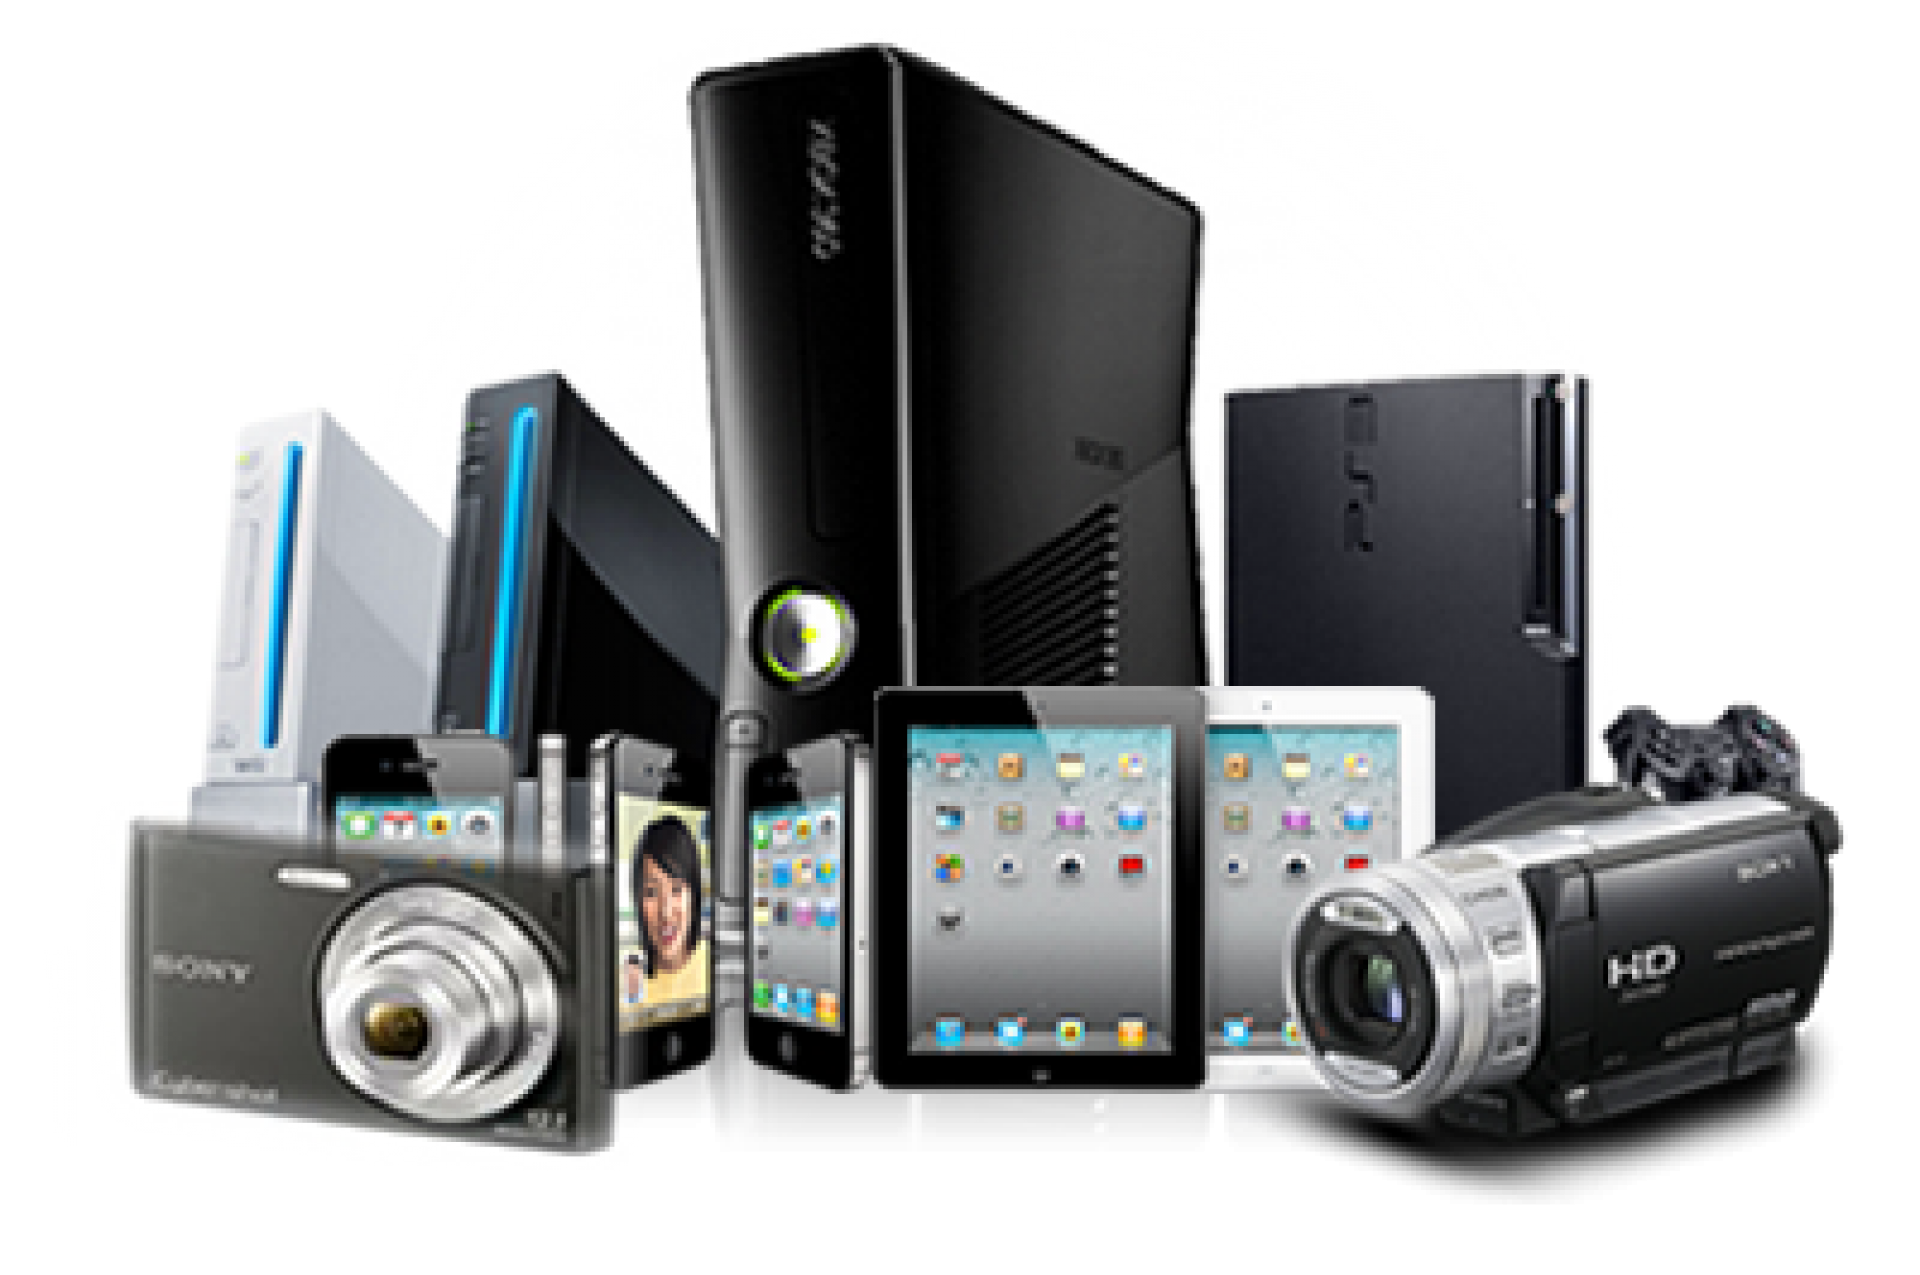
\includegraphics[height=4cm, keepaspectratio,left]{img/introducao/equip_conj_008.png}

\column{0.6\textwidth}

    \begin{itemize}
        \vspace{8pt} 
        \item Circuitos Integrados Modernos:
        \begin{itemize}
            \itemsep8pt 
            \item \textbf{Milhões} de elementos síncronos 
            \item \textbf{Tempo} de projeto \textbf{limitado}
            \item Diversas \textbf{métricas} e \textbf{restrições}
            \item[$\Rightarrow$] \color{blue}{\textbf{Ferramentas de Eletronic Design Automation (EDA) são obrigatórias}}
        \end{itemize}
        % \item Ferramentas de EDA devem aproveitar \textbf{otimizações de software} como:
        % \begin{itemize}
        %     \item uso de melhores estruturas de dados
        %     \item \textbf{exploração da localidade da Cache}
        %     \item paralelismo
        % \end{itemize}
    \end{itemize}

\end{columns}

\end{frame}

\begin{frame}{Fluxo do Projeto de um Circuito Integrado}
    
    \pgfdeclareimage[width=0.65\linewidth]{step1}{img/introducao/step1.pdf}
    \pgfdeclareimage[width=0.65\linewidth]{step2}{img/introducao/step2.pdf}
    
    \begin{center}
        \pgfuseimage<1>{step1}
        \pgfuseimage<2>{step2}
    \end{center}
    
\end{frame}

\begin{frame}{ \textit{Engines} modernas de jogos $\times$ EDA }

\pgfdeclareimage[width=0.35\linewidth]{games2}{img/introducao/games_2.pdf}
\pgfdeclareimage[width=0.35\linewidth]{circuit}{img/introducao/circuits.pdf}

\begin{columns}
\begin{column}{0.5\textwidth}
    \begin{center}
    \pgfuseimage<1>{games2}
    \begin{itemize}
        \item Processa grande quantidade de dado
        \item Renderiza gráficos de alta resolução
    \end{itemize}
    \end{center}
\end{column}
\begin{column}{0.5\textwidth} 
    \begin{center}
        \pgfuseimage<1>{circuit}
        \begin{itemize}
        \item Processa grande quantidade de dados
        \item Otimiza diversas métricas
    \end{itemize}
     \end{center}
\end{column}
\end{columns}

\end{frame}

\begin{frame}{}
    \begin{itemize}
        \itemsep15pt 
        \item[$\Rightarrow$] Ferramentas de EDA devem explorar \textbf{otimizações de software} como:
        \begin{itemize}
            \item Uso de melhores estruturas de dados
                \begin{itemize}
                    \item Árvores Espaciais
                \end{itemize}
            \item \textbf{Exploração da localidade da Cache}
            \item Paralelismo
        \end{itemize}
    \end{itemize}
    
    \pgfdeclareimage[width=0.2\linewidth]{arvore}{img/introducao/3dtree.png}
    \pgfdeclareimage[width=0.3\linewidth]{cache}{img/introducao/cache_locality.png}
    \pgfdeclareimage[width=0.36\linewidth]{paralelismo}{img/introducao/openMP.png}
    
    \vspace{1cm}
    
    \begin{columns}
        \column{0.25\textwidth}
            \centering
            \pgfuseimage<1>{arvore}
        \column{0.36\textwidth}
            \centering
            \pgfuseimage<1>{cache}
        \column{0.38\textwidth}
            \centering
            \pgfuseimage<1>{paralelismo}
    \end{columns}
    
    
\begin{tikzpicture}[remember picture,overlay]
        % \node[rectangle, draw, minimum width = 2.cm, minimum height = 1.cm, color=red, rounded corners, very thick](window)at(1.45,2.55){};
        \node (window)at(1.5,-0.2){\fontsize{3}{5}\selectfont Fonte: https://en.wikipedia.org/wiki/K-d\_tree};
        \node (window1)at(6,-0.2){\fontsize{3}{5}\selectfont Fonte: http://archive.arstechnica.com/paedia/c/caching/m-caching-2.html};
        \node (window2)at(11.7,-0.2){\fontsize{3}{5}\selectfont Fonte: http://csd.ru/soft/version\_116841.html};
    \end{tikzpicture}
    
\end{frame}

% \begin{frame}{Entendendo a hierarquia de memória}

    % \pgfdeclareimage[width=0.8\linewidth]{memory1}{img/introducao/memoryHierarchy.pdf}
    
    % \vspace{15pt}
    
    % \begin{center}
        % \pgfuseimage<1>{memory1}
    % \end{center}

% \end{frame}

% \begin{frame}{Cache com mapeamento direto}

%     \pgfdeclareimage[width=0.55\linewidth]{memory}{img/introducao/mapeamentoMemoria.pdf}
    
%     \begin{itemize}
%         \item Considerando:
%         \begin{itemize}
%             \item palavra de 4 bytes
%             \item bloco de 128 bytes
%         \end{itemize}
%     \end{itemize}
    
%     \vspace{-15pt}
    
%     \begin{center}
%         \pgfuseimage<1>{memory}
%     \end{center}

% \end{frame}


% \begin{frame}{How Object-Oriented Design (OOD) Leads to More Cache Misses}
% \begin{frame}{Como Vector of Structure causa mais \textit{Cache Misses}}
\begin{frame}{Impacto do uso de \textbf{Vector of Structure} no número de \textit{Cache Misses}}
    \begin{itemize}
        \item[] \textbf{Objetivo:} iterar sobre todas as posições dos registradores
    \end{itemize}

    \pgfdeclareimage[width=\linewidth]{ood1}{img/introducao/ood_memory_layout_1.pdf}
    \pgfdeclareimage[width=\linewidth]{ood15}{img/introducao/ood_memory_layout_1_5.pdf}
    % \pgfdeclareimage[width=\linewidth]{ood2}{img/introducao/ood_memory_layout_2.pdf}
    \pgfdeclareimage[width=\linewidth]{ood3}{img/introducao/ood_memory_layout_3.pdf}
    \begin{center}
        \pgfuseimage<1>{ood1}
        \pgfuseimage<2>{ood15}
        % \pgfuseimage<2>{ood2}
        \pgfuseimage<3>{ood3}
    \end{center}
    
    % \only<1-2>{
    % \begin{flushright} 
    %     \color{white}{\LARGE{$\mathbf{50\%}$\textbf{ wasted cache}} \ \ \ \ \ \ }      
    % \end{flushright}
    % }
    % \only<3>{
    % \begin{flushright} 
    %     \color{red}{\LARGE{$\mathbf{50\%}$\textbf{ wasted cache}} \ \ \ \ \ \ }      
    % \end{flushright}
    % }
% Show the memory footprint when iterating over the cells
% data miss
% instruction miss (if updating every cell location)
\end{frame}

\begin{frame}{Vector of Structures x Structure of Vectors}
    \begin{columns}
        \column{.49\linewidth}
            \begin{itemize}
                \item Vector of Structures
                \begin{itemize}
                    \item Object-Oriented Design (OOD)
                \end{itemize}
            \end{itemize}
            \pgfdeclareimage[width=\linewidth]{vecOfStruct}{img/introducao/vectorOfStructure.pdf}
            \begin{center}
                \pgfuseimage<1>{vecOfStruct}
            \end{center}
        \column{.50\linewidth}
            \begin{itemize}
                \item Structure of Vectors
                \begin{itemize}
                    \item Data-Oriented Design (DOD)
                \end{itemize}
            \end{itemize}
            \pgfdeclareimage[width=\linewidth]{structOfVec}{img/introducao/structureOfVectors.pdf}
            \begin{center}
                \pgfuseimage<1>{structOfVec}
            \end{center}
    \end{columns}
\end{frame}

% \begin{frame}{How Data-Oriented Design (DOD) Improves Cache Locality}
\begin{frame}{Como Structure of Vectors melhora a localidade da Cache}
    \begin{itemize}
        \item[] \textbf{Objetivo:} iterar sobre todas as posições dos registradores
    \end{itemize}

    \pgfdeclareimage[width=\linewidth]{dod1}{img/introducao/dod_memory_layout_1.pdf}
    % \pgfdeclareimage[width=0.98\linewidth]{dod2}{img/introducao/dod_memory_layout_2.pdf}
    \pgfdeclareimage[width=0.98\linewidth]{dod3}{img/introducao/dod_memory_layout_3.pdf}
    \begin{center}
        \pgfuseimage<1>{dod1}
        % \pgfuseimage<2>{dod2}
        \pgfuseimage<2>{dod3}
    \end{center}
    
    % \only<1-2>{
    % \begin{flushright} 
    %     \color{white}{\LARGE{$\mathbf{100\%}$\textbf{ used cache}} \ \ \ \ \ \ } 
    % \end{flushright}
    % }
    % \only<3>{
    % \begin{flushright} 
    %     \color{eclgreen}{\LARGE{$\mathbf{100\%}$\textbf{ used cache}} \ \ \ \ \ \ } 
    % \end{flushright}
    % }
% Show the memory footprint when iterating over the cells
% data miss
% instruction miss (if updating every cell location)
\end{frame}

\section{Trabalhos Correlatos}
\subsection*{}

% tabela de trabalhos

\begin{frame}{Trabalhos correlatos}
    
    \only<1>{
        \begin{table}[]
        \centering
        \resizebox{\textwidth}{!}{%
            \begin{tabular}{@{}ccccc@{}}
            \toprule
            Trabalho & Momento da Otimização & Consideração da Cache & Técnica & Casos de Uso \\ \midrule
            Majeti, 2013 & Compilação & Cache-Aware & \begin{tabular}[c]{@{}c@{}}inserção de metadados\\  no código fonte\end{tabular} & sintéticos \\[12pt]
            Li, 2014 & Compilação & Cache-Oblivious & reordenamento das instruções & SPEC2006 CPU \\[9pt]
            Tang, 2015 & Pós-Compilação & Cache-Oblivious & \begin{tabular}[c]{@{}c@{}}removem dependencias \\ na Programação Dinâmica\end{tabular} & sintéticos \\[12pt]
            Qasem, 2017 & Pós-Compilação & Cache-Oblivious & propõem Compressed-Array & sintéticos \\[9pt]
            Este Trabalho & Pré-Compilação & Cache-Oblivious & \begin{tabular}[c]{@{}c@{}}Data-Oriented Design\\ com Entity Component System\end{tabular} & \begin{tabular}[c]{@{}c@{}}3 algoritmos de\\ Physical Design*\end{tabular} \\[9pt] \midrule
            \multicolumn{5}{l}{* Entrada realista oriunda de circuitos industriais providos pela competição ICCAD2015.} \\ \bottomrule
            \end{tabular}
        }
        \end{table}
    }
    \only<2>{
        \begin{table}[]
        \centering
        \resizebox{\textwidth}{!}{%
            \begin{tabular}{@{}ccccc@{}}
            \toprule
            Trabalho & Momento da Otimização & Consideração da Cache & Técnica & Casos de Uso \\ \midrule
            \rowcolor{green!40} Majeti, 2013 & Compilação & Cache-Aware & \begin{tabular}[c]{@{}c@{}}inserção de metadados\\  no código fonte\end{tabular} & sintéticos \\[12pt]
            \rowcolor{green!40} Li, 2014 & Compilação & Cache-Oblivious & reordenamento das instruções & SPEC2006 CPU \\[9pt]
            Tang, 2015 & Pós-Compilação & Cache-Oblivious & \begin{tabular}[c]{@{}c@{}}removem dependencias \\ na Programação Dinâmica\end{tabular} & sintéticos \\[12pt]
            Qasem, 2017 & Pós-Compilação & Cache-Oblivious & propõem Compressed-Array & sintéticos \\[9pt]
            Este Trabalho & Pré-Compilação & Cache-Oblivious & \begin{tabular}[c]{@{}c@{}}Data-Oriented Design\\ com Entity Component System\end{tabular} & \begin{tabular}[c]{@{}c@{}}3 algoritmos de\\ Physical Design*\end{tabular} \\[9pt] \midrule
            \multicolumn{5}{l}{* Entrada realista oriunda de circuitos industriais providos pela competição ICCAD2015.} \\ \bottomrule
            \end{tabular}
        }
        \end{table}
    }
    \only<3>{
        \begin{table}[]
        \centering
        \resizebox{\textwidth}{!}{%
            \begin{tabular}{@{}ccccc@{}}
            \toprule
            Trabalho & Momento da Otimização & Consideração da Cache & Técnica & Casos de Uso \\ \midrule
            Majeti, 2013 & Compilação & Cache-Aware & \begin{tabular}[c]{@{}c@{}}inserção de metadados\\  no código fonte\end{tabular} & sintéticos \\[12pt]
            Li, 2014 & Compilação & Cache-Oblivious & reordenamento das instruções & SPEC2006 CPU \\[9pt]
            \rowcolor{green!40} Tang, 2015 & Pós-Compilação & Cache-Oblivious & \begin{tabular}[c]{@{}c@{}}removem dependencias \\ na Programação Dinâmica\end{tabular} & sintéticos \\[12pt]
            \rowcolor{green!40} Qasem, 2017 & Pós-Compilação & Cache-Oblivious & propõem Compressed-Array & sintéticos \\[9pt]
            Este Trabalho & Pré-Compilação & Cache-Oblivious & \begin{tabular}[c]{@{}c@{}}Data-Oriented Design\\ com Entity Component System\end{tabular} & \begin{tabular}[c]{@{}c@{}}3 algoritmos de\\ Physical Design*\end{tabular} \\[9pt] \midrule
            \multicolumn{5}{l}{* Entrada realista oriunda de circuitos industriais providos pela competição ICCAD2015.} \\ \bottomrule
            \end{tabular}
        }
        \end{table}
    }
    \only<4>{
        \begin{table}[]
        \centering
        \resizebox{\textwidth}{!}{%
            \begin{tabular}{@{}ccccc@{}}
            \toprule
            Trabalho & Momento da Otimização & Consideração da Cache & Técnica & Casos de Uso \\ \midrule
            Majeti, 2013 & Compilação & Cache-Aware & \begin{tabular}[c]{@{}c@{}}inserção de metadados\\  no código fonte\end{tabular} & sintéticos \\[12pt]
            Li, 2014 & Compilação & Cache-Oblivious & reordenamento das instruções & SPEC2006 CPU \\[9pt]
            Tang, 2015 & Pós-Compilação & Cache-Oblivious & \begin{tabular}[c]{@{}c@{}}removem dependencias \\ na Programação Dinâmica\end{tabular} & sintéticos \\[12pt]
            Qasem, 2017 & Pós-Compilação & Cache-Oblivious & propõem Compressed-Array & sintéticos \\[9pt]
            \rowcolor{green!40} Este Trabalho & Pré-Compilação & Cache-Oblivious & \begin{tabular}[c]{@{}c@{}}Data-Oriented Design\\ com Entity Component System\end{tabular} & \begin{tabular}[c]{@{}c@{}}3 algoritmos de\\ Physical Design*\end{tabular} \\[9pt] \midrule
            \multicolumn{5}{l}{* Entrada realista oriunda de circuitos industriais providos pela competição ICCAD2015.} \\ \bottomrule
            \end{tabular}
        }
        \end{table}
    }
\end{frame}
\section{Técnica Proposta}
\subsection*{}

% apresenta dod
% apresenta padrão entity system
% apresenta implementações
% apresenta os 3 problemas que serão tratados


\begin{frame}{Organização dos dados proposta}

    \vspace{1cm}

    \begin{itemize}
        \item \textbf{Data-Oriented Design} (DOD)
        \begin{itemize}
            \item Focado na organização dos dados
            \item Otimização do uso da memória cache
        \end{itemize}
        \item \textbf{Entity-Component System} (ECS)
        \begin{itemize}
            \item \textbf{Padrão de projeto} utilizado principalmente no desenvolvimento de jogos
            \item Baseado em \textbf{Entidades} e \textbf{Propriedades} (Componentes)
        \end{itemize}
    \end{itemize}

    \pgfdeclareimage[width=0.4\linewidth]{entity}{img/tecnica/entity.pdf}
    % \pgfdeclareimage[width=0.7\linewidth]{entity_pin}{img/tecnica/pin_dod.pdf}

    \begin{center}
        \pgfuseimage<1>{entity}
        % \pgfuseimage<2>{entity_pin}
    \end{center}

\end{frame}

\begin{frame}{Organização dos dados proposta}
    \begin{columns}
        \column{.45\linewidth}
            \pgfdeclareimage[width=\linewidth]{fig1}{img/tecnica/registerClusterclassOOD.pdf}
            \begin{itemize}
                \item Object-Oriented Design
            \end{itemize}
            \pgfuseimage<1>{fig1}
        \column{.5\linewidth}
            \pgfdeclareimage[width=\linewidth]{fig2}{img/tecnica/propertiesDOD.pdf}
            \begin{itemize}
                \item Data-Oriented Design
            \end{itemize}
            \pgfuseimage<1>{fig2}
    \end{columns}
\end{frame}




\begin{frame}{Operações: busca, adição, e remoção de entidades em $\mathcal{O}(1)$}

\pgfdeclareimage[width=0.9\linewidth]{es1}{img/tecnica/entitySystemInsertion_1.pdf}
\pgfdeclareimage[width=0.9\linewidth]{es2}{img/tecnica/entitySystemInsertion_2.pdf}
\pgfdeclareimage[width=0.7\linewidth]{es3}{img/tecnica/entitySystemInsertion_3.pdf}
\pgfdeclareimage[width=0.7\linewidth]{es31}{img/tecnica/entitySystemInsertion_3_1.pdf}
\pgfdeclareimage[width=0.7\linewidth]{mask}{img/tecnica/mask.pdf}

\only<1>{
    \begin{itemize}
        \item \textbf{Busca}: $\mathcal{O}(1)$
    \end{itemize}
    \begin{center}
        \pgfuseimage{es1}
    \end{center}
}
\only<2>{
    \begin{itemize}
        \item \textbf{Adição}: $\mathcal{O}(1)$
    \end{itemize}
    \begin{center}
        \pgfuseimage{es2}
    \end{center}
}
\only<3>{
    \vspace{0.5cm}
    \begin{itemize}
        \item \textbf{Remoção}: $\mathcal{O}(1)$
    \end{itemize}
    \vspace{-0.5cm}
    \begin{center}
        \pgfuseimage{es31}
        
        \vspace{0.5cm}
        
        \pgfuseimage{mask}
    \end{center}
}
\only<4>{
    \vspace{0.5cm}
    \begin{itemize}
        \item \textbf{Remoção}: $\mathcal{O}(1)$
    \end{itemize}
    \vspace{-0.5cm}
    \begin{center}
        \pgfuseimage{es31}
        
        \vspace{0.5cm}
        
        \pgfuseimage{es3}
    \end{center}
}

% \begin{center}
    % \pgfuseimage<1>{es1}
    % \pgfuseimage<2>{es2}
    % \pgfuseimage<3>{es3}
% \end{center}

\end{frame}

% \begin{frame}{Relationships Between Entities: aggregation and composition}

% \pgfdeclareimage[width=0.75\linewidth]{es1}{img/tecnica/aggregation_composition_1.pdf}
% \pgfdeclareimage[width=0.75\linewidth]{es2}{img/tecnica/aggregation_composition_2.pdf}
% \pgfdeclareimage[width=0.75\linewidth]{es3}{img/tecnica/aggregation_composition_3.pdf}
% \pgfdeclareimage[width=0.75\linewidth]{es4}{img/tecnica/aggregation_composition_4.pdf}

% \vspace{10pt}

% \begin{center}

% \pgfuseimage<1>{es1}
% \pgfuseimage<2>{es2}
% \pgfuseimage<3>{es3}
% \pgfuseimage<4>{es4}

% \end{center}

% \end{frame}

% \begin{frame}{Aggregation code example}

    
%     \begin{figure}
%         \centering
%         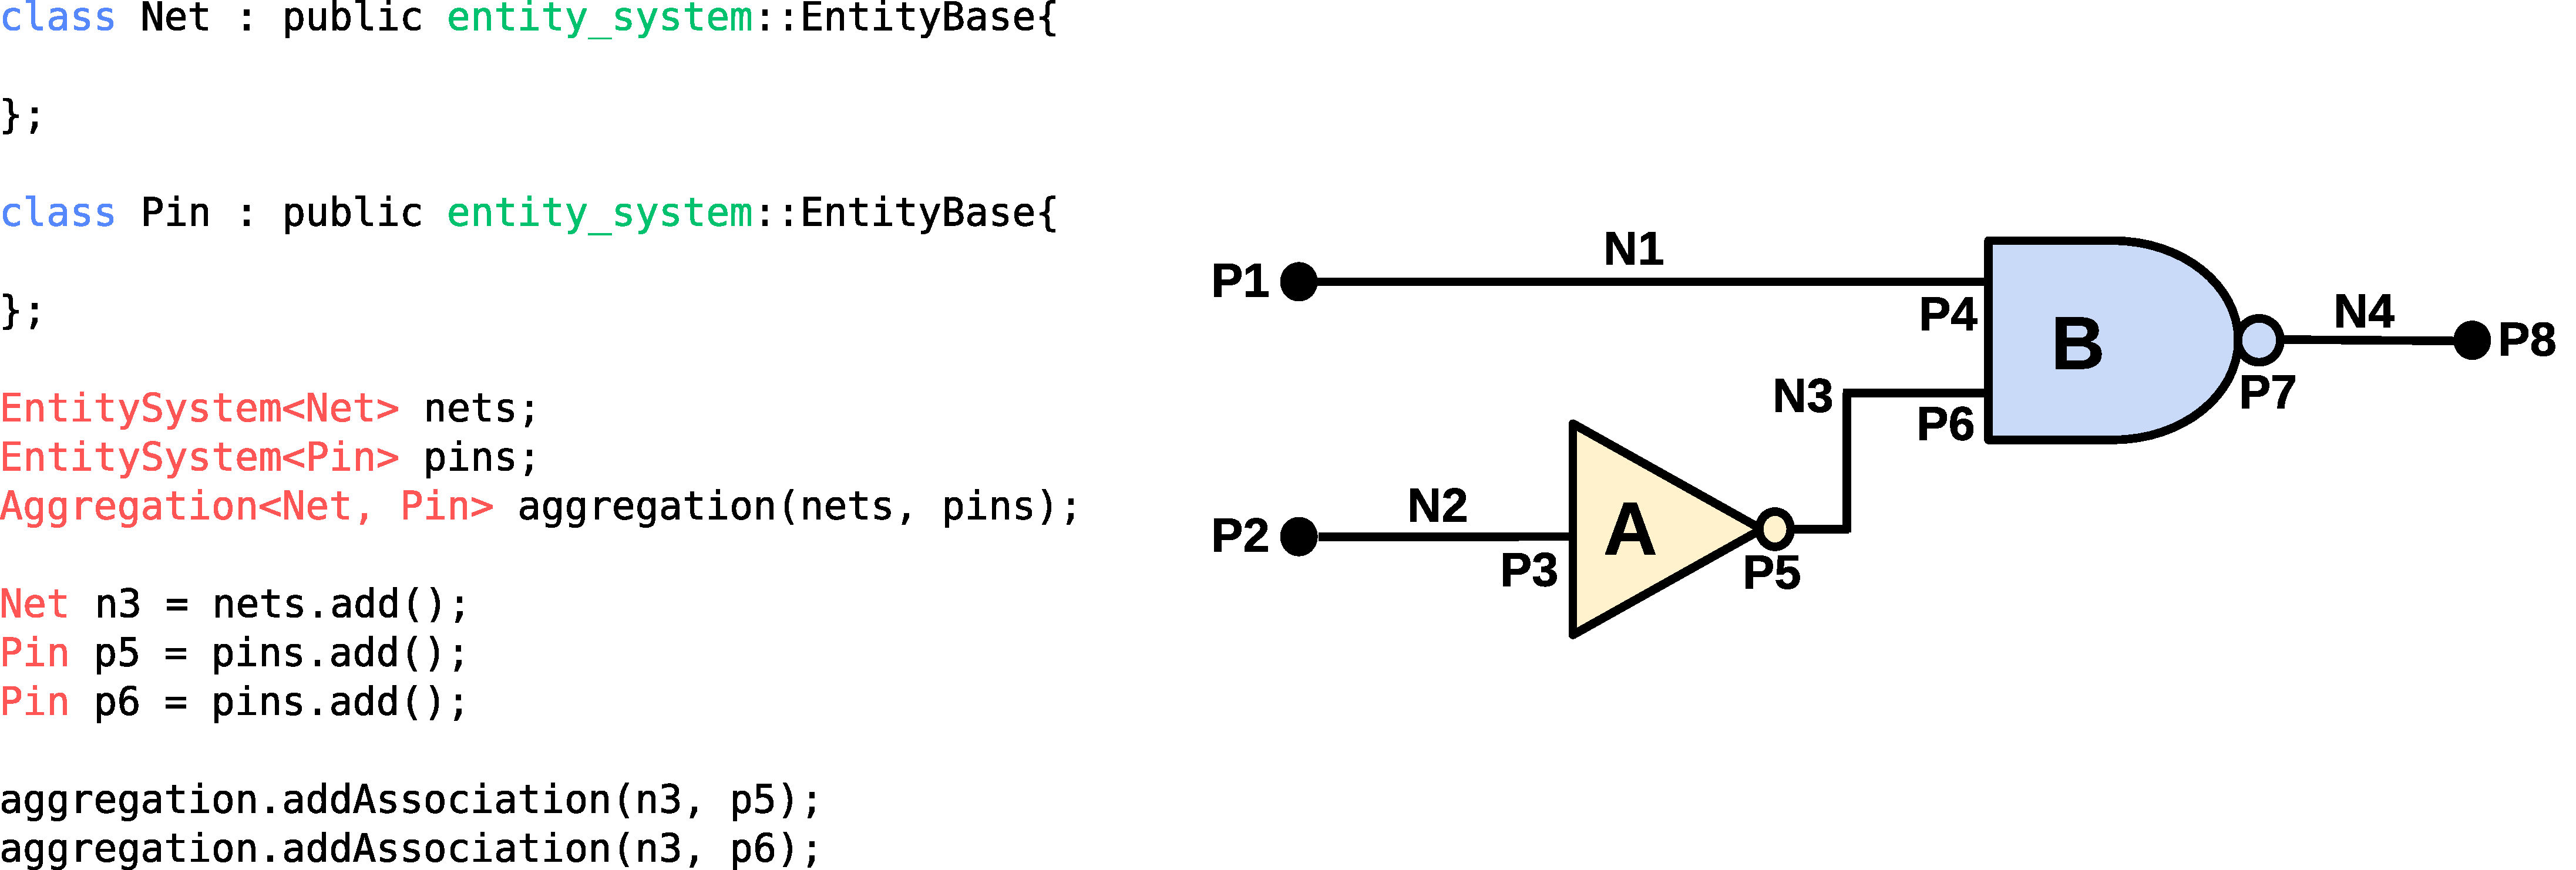
\includegraphics[width=\textwidth]{img/tecnica/code_example_aggregation.pdf}
%     \end{figure}

% \end{frame}

% \begin{frame}{Composition code example}

    
%     \begin{figure}
%         \centering
%         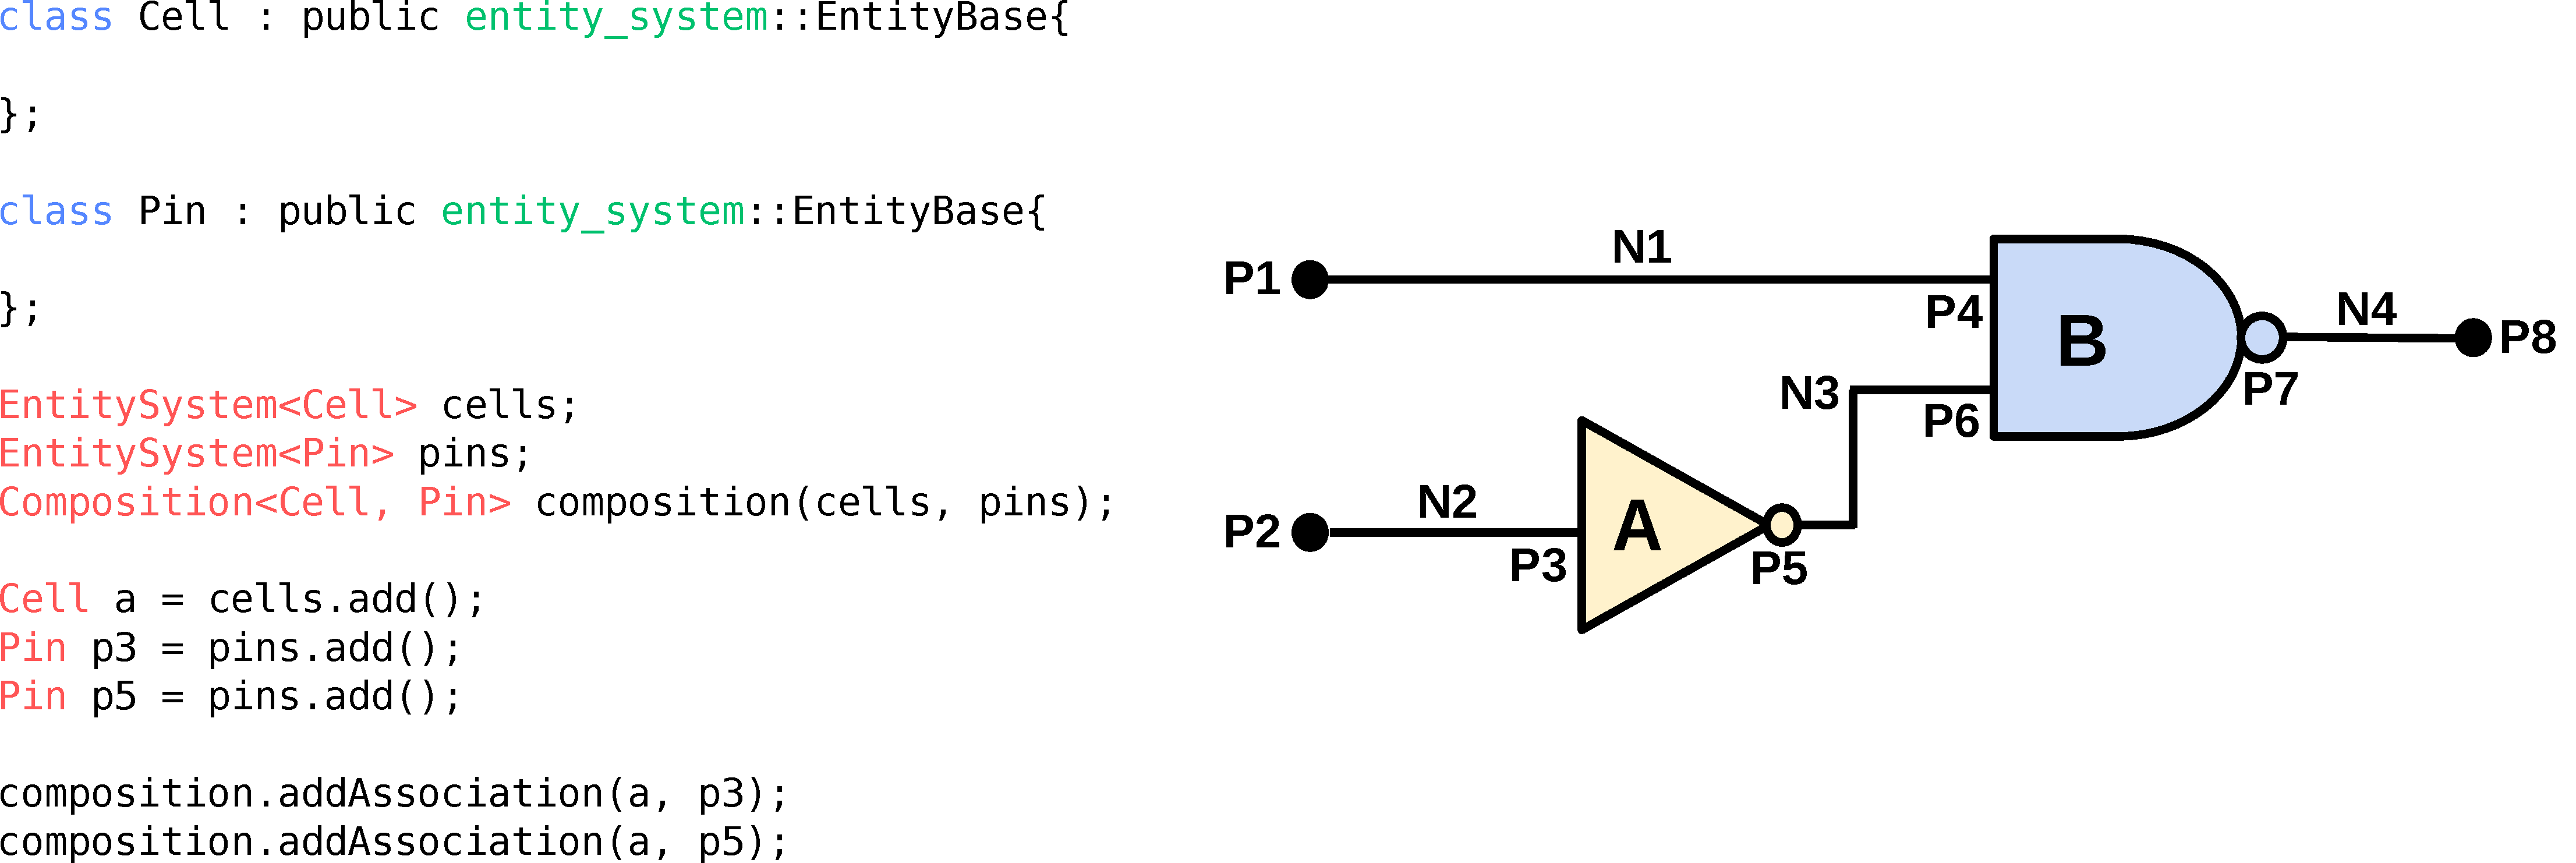
\includegraphics[width=\textwidth]{img/tecnica/code_example_composition.pdf}
%     \end{figure}

% \end{frame}


% ---------------------------------------------------------------------------------------------------------

\section{Metodologia e Resultados Preliminares}
\subsection*{}

\begin{frame}{Metodologia}
    \begin{itemize}
        \item Avaliar:
        \begin{itemize}
            \item Número de \textbf{\textit{Cache Misses}}
            \item Tempo de execução
        \end{itemize}
        \item 3 algoritmos de Physical Design:
        \begin{itemize}
            \item Problema A: Verificar limites do chip
            \item Problema B: Estimar o tamanho das interconexões
            \item Problema C: Clusterização de elementos
        \end{itemize}
        \item Implementações:
        \begin{itemize}
            \item Abordagem tradicional: Object-Oriented Design (OOD)
            \item Abordagem proposta: Data-Oriented Design (DOD) 
        \end{itemize}
    \end{itemize}
\end{frame}

\begin{frame}{Infraestrutura}
     \begin{columns}
        \column{.6\linewidth}
        
            \begin{itemize}
                % \itemsep15pt 
                \item Ophidian
                \item ICCAD 2015 CAD Contest: 
                \begin{itemize}
                    \item 8 circuitos de tamanhos de \\ \textbf{768m} a \textbf{1.93M} de células
                \end{itemize}
                \item Linux workstation com processador Intel\textsuperscript{\textregistered} Core\textsuperscript{\textregistered} i5-4460 @ 3.20~GHz
                \begin{itemize}
                    \item 32GB~RAM (DDR3 @ 1600MHz)
                    \item Memória Cache:
                        \begin{itemize}
                            \item L1: 64KB
                            \item L2: 256KB
                            \item L3: 6144KB
                        \end{itemize}
                \end{itemize}
                \item 30 repetições para garantir um pequeno intervalo de confiança
                % \item Código fonte e experimentos disponíveis na Ophidian %\footnote{Disponível em: https://github.com/eclufsc/ophidian}
                % \item \textbf{Scenario ~A}: check if all circuit cells' positions lie within the circuit's boundaries
                % In this scenario only one property is necessary for each entity (cell position), so it fully explores the data locality provided by \ac{dod}.
                % \item \textbf{Scenario ~B}: computing the interconnection wirelength for all circuit nets
                % This scenario accesses different properties of different entities. Therefore, it cannot efficiently explore the data locality provided by \ac{dod}, since the properties of the pins in a single net may not be contiguous in memory, unless the property array is previously sorted.
            \end{itemize}
            
        \column{.4\linewidth}
            \pgfdeclareimage[width=\linewidth]{mr1}{img/results/architectureMemoryZeus.pdf}
            \begin{center}
                \pgfuseimage<1>{mr1}
            \end{center}
    \end{columns}
\end{frame}

\begin{frame}{Problema A: Verificar limites do chip}
    
    \pgfdeclareimage[width=0.3\linewidth]{problema}{img/tecnica/problemaA.pdf}
    \pgfdeclareimage[width=0.27\linewidth]{ood}{img/tecnica/classHierarchyChipBoundariesOOD.pdf}
    \pgfdeclareimage[width=0.5\linewidth]{dod}{img/tecnica/chipBoundariesDOD.pdf}

    \begin{minipage}[c][.3\textheight][c]{1\textwidth}
        \centering
        \vspace{1cm}
        \pgfuseimage<1>{problema}
    \end{minipage}
    \begin{minipage}[c][.7\textheight][c]{1\textwidth}
        \begin{columns}
            \column{.5\linewidth}
                \vspace{1cm}
                \begin{itemize}
                    \item Object-Oriented Design
                \end{itemize}
                \centering
                \vspace{.5cm}
                \pgfuseimage<1>{ood}
                \vspace{1.2cm}
            \column{.5\linewidth}
                \vspace{-2.5cm}
                \begin{itemize}
                    \item Data-Oriented Design
                \end{itemize}
                \vspace{0.5cm}
                \pgfuseimage<1>{dod}
        \end{columns}
    \end{minipage}
    
\end{frame}

\begin{frame}{Problema A: Verificar limites do chip}

    \pgfdeclareimage[width=0.5\linewidth]{miss_1}{img/results/miss_problem_A_1.pdf}
    \pgfdeclareimage[width=0.5\linewidth]{miss_2}{img/results/miss_problem_A_2.pdf}
    \pgfdeclareimage[width=0.5\linewidth]{runtime_1}{img/results/runtime_problem_A_1.pdf}
    \pgfdeclareimage[width=0.5\linewidth]{runtime_2}{img/results/runtime_problem_A_2.pdf}

    \begin{columns}
        \column{.5\linewidth}
            \only<1>{
                \centering
                Cache Misses
                
                \vspace{0.5cm}
                \pgfuseimage{miss_1}
            }
            \only<2-4>{
                \centering
                Cache Misses
                
                \vspace{0.5cm}
                \pgfuseimage{miss_2}
            }
        \column{.5\linewidth}
            \only<3>{
                \centering
                Tempo de execução
                
                \vspace{0.5cm}
                \pgfuseimage{runtime_1}
            }
            \only<4>{
                \centering
                Tempo de execução
                
                \vspace{0.5cm}
                \pgfuseimage{runtime_2}
            }
    \end{columns}
\end{frame}

\begin{frame}{Problema B: Estimar o tamanho das interconexões}

    \pgfdeclareimage[width=0.15\linewidth]{problema}{img/tecnica/problemaB.pdf}
    \pgfdeclareimage[width=0.3\linewidth]{ood}{img/tecnica/classHierarchyOOD.pdf}
    \pgfdeclareimage[width=0.5\linewidth]{dod}{img/tecnica/estimativa_interconection_dod.pdf}

    \begin{minipage}[c][.3\textheight][c]{1\textwidth}
        \centering
        \vspace{1.4cm}
        \pgfuseimage<1>{problema}
    \end{minipage}
    \begin{minipage}[c][.7\textheight][c]{1\textwidth}
        \begin{columns}
            \column{.5\linewidth}
                \begin{itemize}
                    \item Object-Oriented Design
                \end{itemize}
                \centering
                % \vspace{.5cm}
                \pgfuseimage<1>{ood}
                % \vspace{1.2cm}
            \column{.5\linewidth}
                \begin{itemize}
                    \item Data-Oriented Design
                \end{itemize}
                \pgfuseimage<1>{dod}
                \vspace{.5cm}
        \end{columns}
    \end{minipage}
        
\end{frame}

\begin{frame}{Problema B: Estimar o tamanho das interconexões}

    \pgfdeclareimage[width=0.5\linewidth]{miss_1}{img/results/miss_problem_B_1.pdf}
    \pgfdeclareimage[width=0.5\linewidth]{miss_2}{img/results/miss_problem_B_2.pdf}
    \pgfdeclareimage[width=0.5\linewidth]{runtime_1}{img/results/runtime_problem_B_1.pdf}
    \pgfdeclareimage[width=0.5\linewidth]{runtime_2}{img/results/runtime_problem_B_2.pdf}

    \begin{columns}
        \column{.5\linewidth}
            \only<1>{
                \centering
                Cache Misses
                
                \vspace{0.5cm}
                \pgfuseimage{miss_1}
            }
            \only<2-4>{
                \centering
                Cache Misses
                
                \vspace{0.5cm}
                \pgfuseimage{miss_2}
            }
        \column{.5\linewidth}
            \only<3>{
                \centering
                Tempo de execução
                
                \vspace{0.5cm}
                \pgfuseimage{runtime_1}
            }
            \only<4>{
                \centering
                Tempo de execução
                
                \vspace{0.5cm}
                \pgfuseimage{runtime_2}
            }
    \end{columns}
\end{frame}

\begin{frame}{Problema B: Estimar o tamanho das interconexões}

    \pgfdeclareimage[width=0.75\linewidth]{future}{img/results/future_work_problem_B.pdf}

    \begin{itemize}
        \item \textbf{Possível otimização}:
        \begin{itemize}
            \item Agrupar a posições dos pinos
        \end{itemize}
    \end{itemize}
    
    \centering
    \pgfuseimage<1>{future}
    
\end{frame}


\begin{frame}{Exemplo HPWL com agrupamento dos pinos}
    \pgfdeclareimage[width=0.8\linewidth]{hpwl0}{img/results/hpwl/hpwl_anim_0.pdf}
    \pgfdeclareimage[width=0.8\linewidth]{hpwl1}{img/results/hpwl/hpwl_anim_1.pdf}
    \pgfdeclareimage[width=0.8\linewidth]{hpwl2}{img/results/hpwl/hpwl_anim_2.pdf}
    \pgfdeclareimage[width=0.8\linewidth]{hpwl3}{img/results/hpwl/hpwl_anim_3.pdf}
    \pgfdeclareimage[width=0.8\linewidth]{hpwl4}{img/results/hpwl/hpwl_anim_4.pdf}
    \pgfdeclareimage[width=0.8\linewidth]{hpwl5}{img/results/hpwl/hpwl_anim_5.pdf}
    \centering
    \vspace{0.5cm}

    \pgfuseimage<1>{hpwl0}
    \pgfuseimage<2>{hpwl1}
    \pgfuseimage<3>{hpwl2}
    \pgfuseimage<4>{hpwl3}
    \pgfuseimage<5>{hpwl4}
    \pgfuseimage<6>{hpwl5}
    
    \begin{tikzpicture}[remember picture,overlay]
        % \node[rectangle, draw, minimum width = 2.cm, minimum height = 1.cm, color=red, rounded corners, very thick](window)at(1.45,2.55){};
        \node (window)at(5.5,6.5){\color{red}{\textbf{Ordem original}}};
        \node (window1)at(5.5,2.9){\color{green}{\textbf{Agrupando pinos}}};
        \node (window2)at(5.5,2.5){\color{green}{\textbf{de uma mesma net}}};
    \end{tikzpicture}
\end{frame}

\begin{frame}{Problema C: Clusterização de elementos}

    \pgfdeclareimage[width=0.2\linewidth]{problema}{img/tecnica/problemaC.pdf}
    \pgfdeclareimage[width=0.3\linewidth]{ood}{img/tecnica/registerClusterclassOOD.pdf}
    \pgfdeclareimage[width=0.5\linewidth]{dod}{img/tecnica/propertiesDOD.pdf}

    % \begin{minipage}[c][.3\textheight][c]{1\textwidth}
    %     \centering
    %     \vspace{1.4cm}
    %     \pgfuseimage<1>{problema}
    % \end{minipage}
    % \begin{minipage}[c][.7\textheight][c]{1\textwidth}
        \begin{columns}
            \column{.5\linewidth}
                \centering
                % \vspace{1.4cm}
                \pgfuseimage<1>{problema}
                \vspace{.5cm}
                \begin{itemize}
                    \item Object-Oriented Design
                \end{itemize}
                % \centering
                % \vspace{.5cm}
                \pgfuseimage<1>{ood}
                % \vspace{1.2cm}
            \column{.5\linewidth}
                \begin{itemize}
                    \item Data-Oriented Design
                \end{itemize}
                \pgfuseimage<1>{dod}
        \end{columns}
    % \end{minipage}
   
    % \begin{columns}
    %     \column{.5\linewidth}
    %         \begin{itemize}
    %             \item Object-Oriented Design
    %         \end{itemize}
    %         \pgfuseimage<1>{ood}
    %     \column{.5\linewidth}
    %         \begin{itemize}
    %             \item Data-Oriented Design
    %         \end{itemize}
    %         \pgfuseimage<1>{dod}
    % \end{columns}

\end{frame}

\begin{frame}{Problema C: Clusterização de elementos }

    \pgfdeclareimage[width=0.5\linewidth]{miss_1}{img/results/miss_problem_C_1_sequential.pdf}
    \pgfdeclareimage[width=0.5\linewidth]{miss_2}{img/results/miss_problem_C_2_sequential.pdf}
    \pgfdeclareimage[width=0.5\linewidth]{runtime_1}{img/results/runtime_problem_C_1_sequential.pdf}
    \pgfdeclareimage[width=0.5\linewidth]{runtime_2}{img/results/runtime_problem_C_2_sequential.pdf}

    \begin{itemize}
        \item Execução \textbf{Sequencial}
    \end{itemize}

    \vspace{0.3cm}

    \begin{columns}
        \column{.5\linewidth}
            \only<1>{
                \centering
                Cache Misses
                
                \vspace{0.5cm}
                \pgfuseimage{miss_1}
            }
            \only<2-4>{
                \centering
                Cache Misses
                
                \vspace{0.5cm}
                \pgfuseimage{miss_2}
            }
        \column{.5\linewidth}
            \only<3>{
                \centering
                Tempo de execução
                
                \vspace{0.5cm}
                \pgfuseimage{runtime_1}
            }
            \only<4>{
                \centering
                Tempo de execução
                
                \vspace{0.5cm}
                \pgfuseimage{runtime_2}
            }
    \end{columns}
\end{frame}

\begin{frame}{Problema C: Clusterização de elementos }

    \pgfdeclareimage[width=0.5\linewidth]{miss_1}{img/results/miss_problem_C_1_parallel.pdf}
    \pgfdeclareimage[width=0.5\linewidth]{miss_2}{img/results/miss_problem_C_2_parallel.pdf}
    \pgfdeclareimage[width=0.5\linewidth]{runtime_1}{img/results/runtime_problem_C_1_parallel.pdf}
    \pgfdeclareimage[width=0.5\linewidth]{runtime_2}{img/results/runtime_problem_C_2_parallel.pdf}

    \begin{itemize}
        \item Execução \textbf{Paralela}
    \end{itemize}

    \vspace{0.3cm}

    \begin{columns}
        \column{.5\linewidth}
            \only<1>{
                \centering
                Cache Misses
                
                \vspace{0.5cm}
                \pgfuseimage{miss_1}
            }
            \only<2-4>{
                \centering
                Cache Misses
                
                \vspace{0.5cm}
                \pgfuseimage{miss_2}
            }
        \column{.5\linewidth}
            \only<3>{
                \centering
                Tempo de execução
                
                \vspace{0.5cm}
                \pgfuseimage{runtime_1}
            }
            \only<4>{
                \centering
                Tempo de execução
                
                \vspace{0.5cm}
                \pgfuseimage{runtime_2}
            }
    \end{columns}
\end{frame}


\section{Cronograma}
\subsection*{}

% o que ja foi feito
% o que falta fazer
% tabela do cronograma

\begin{frame}{Atividades concluídas}
    \begin{itemize}
        \item \textbf{C1}: Implementar problemas de \textit{Physical Design} utilizando OOD e DOD;
        \item \textbf{C2}: Avaliar quantitativamente os resultados obtidos na Atividade C1;
        \item \textbf{C3}: Escrita e submissão do artigo para o ISPD 2017 (Qualis  CC 2016: B1);
        \item \textbf{C4}: Implementar técnica de clusterização de elementos utilizando OOD e DOD;
        \item \textbf{C5}: Avaliar quantitativamente os resultados obtidos na Atividade C4;
        \item \textbf{C6}: Escrita e submissão do artigo para o SBCCI 2017 (Qualis  CC 2016: B2);
        \item \textbf{C7}: Apresentação do artigo no SBCCI 2017;
        \item \textbf{C8}: Escrita do texto do Exame de Qualificação.
    \end{itemize}
\end{frame}

\begin{frame}{Publicações}

    \begin{itemize}
        % \itemsep15pt 
        \item Artigos:
        \begin{enumerate}
            \itemsep15pt 
            \item How Game Engines Can Inspire EDA Tools Development: A use case for an open-source physical design library
            \begin{itemize}
                \item \textbf{Evento}: International Symposium on Physical Design (ISPD 2017)
                % \item Ano: 2017
                \item \textbf{Qualis} (CC 2016): B1
            \end{itemize}
            \item Exploiting Cache Locality to Speedup Register Clustering
            \begin{itemize}
                \item \textbf{Evento}: 30th Symposium on Integrated Circuits and Systems Design (SBCCI 2017)
                % \item Ano: 2017
                \item \textbf{Qualis} (CC 2016): B2
            \end{itemize}
        \end{enumerate}
        % \item Prêmio:
        % \begin{itemize}
        %     \item 2017 CAD Contest (Problem C: Multi-Deck Standard Cell Legalization)
        %     \begin{itemize}
        %         \item \textbf{Colocação}: TOP 3 (resultado oficial será divulgado no ICCAD dia 13 de Novembro de 2017)
        %         \item \textbf{Melhor runtime} dentre os competidores (testes alpha e beta)
        %         \item \textbf{Equipe}: Ophidian
        %         \item \textbf{Membros}: Renan Netto, Tiago Fontana, Sheiny Fabre, Thiago Barbatto, Chrystian Guth, Prof. José Güntzel e Prof. Laercio Lima Pilla
        %     \end{itemize}
        % \end{itemize}
    \end{itemize}
    
\end{frame}

\begin{frame}{Atividades pendentes}
    \begin{itemize}
        \item \textbf{P1}: Realizar as sugestões de melhoria do exame de qualificação;
        \item \textbf{P2}: Implementar Sistema de Entidade com suporte ao agrupamento das propriedades de uma entidade;
        \item \textbf{P3}: Adaptar problemas já implementados;
        \item \textbf{P4}: Avaliar quantitativamente os resultados obtidos na Atividade P3;
        \item \textbf{P5}: Submeter artigo para revista ou evento com as contribuições totais deste trabalho (ICCAD 2018);
        \item \textbf{P6}: Escrever a dissertação de mestrado;
        \item \textbf{P7}: Preparar a apresentação e defender este trabalho de mestrado;
        \item \textbf{P8}: Realizar as correções sugeridas pela banca durante a defesa;
        \item \textbf{P9}: Entregar da dissertação de mestrado.
    \end{itemize}
\end{frame}

\begin{frame}{Cronograma}
    \begin{table}[]
        \centering
        % \caption[Cronograma do trabalho]{Cronograma previsto para realização do trabalho de mestrado}
        \label{tab:cronograma}
        \resizebox{\textwidth}{!}{
        \begin{tabular}{@{}cccccccccc@{}}
        \toprule
                                          & \textbf{Novembro}      & \textbf{Dezembro}      & \textbf{Janeiro}       & \textbf{Fevereiro}     & \textbf{Março}         & \textbf{Abril}         & \textbf{Maio}          & \textbf{Junho}         & \textbf{Julho}         \\ \midrule
        \multicolumn{1}{|l|}{\textbf{P1:} Correções EQM} & \multicolumn{1}{c|}{X} & \multicolumn{1}{c|}{}  & \multicolumn{1}{c|}{}  & \multicolumn{1}{c|}{}  & \multicolumn{1}{c|}{}  & \multicolumn{1}{c|}{}  & \multicolumn{1}{c|}{}  & \multicolumn{1}{c|}{}  & \multicolumn{1}{c|}{}  \\ \midrule
        \multicolumn{1}{|l|}{\textbf{P2:} Implementação} & \multicolumn{1}{c|}{}  & \multicolumn{1}{c|}{X} & \multicolumn{1}{c|}{X} & \multicolumn{1}{c|}{}  & \multicolumn{1}{c|}{}  & \multicolumn{1}{c|}{}  & \multicolumn{1}{c|}{}  & \multicolumn{1}{c|}{}  & \multicolumn{1}{c|}{}  \\ \midrule
        \multicolumn{1}{|l|}{\textbf{P3:} Adaptação} & \multicolumn{1}{c|}{}  & \multicolumn{1}{c|}{X} & \multicolumn{1}{c|}{X} & \multicolumn{1}{c|}{X} & \multicolumn{1}{c|}{}  & \multicolumn{1}{c|}{}  & \multicolumn{1}{c|}{}  & \multicolumn{1}{c|}{}  & \multicolumn{1}{c|}{}  \\ \midrule
        \multicolumn{1}{|l|}{\textbf{P4:} Avaliação Resultados} & \multicolumn{1}{c|}{}  & \multicolumn{1}{c|}{X} & \multicolumn{1}{c|}{X} & \multicolumn{1}{c|}{X} & \multicolumn{1}{c|}{}  & \multicolumn{1}{c|}{}  & \multicolumn{1}{c|}{}  & \multicolumn{1}{c|}{}  & \multicolumn{1}{c|}{}  \\ \midrule
        \multicolumn{1}{|l|}{\textbf{P5:} Artigo} & \multicolumn{1}{c|}{}  & \multicolumn{1}{c|}{}  & \multicolumn{1}{c|}{}  & \multicolumn{1}{c|}{}  & \multicolumn{1}{c|}{X} & \multicolumn{1}{c|}{X} & \multicolumn{1}{c|}{}  & \multicolumn{1}{c|}{}  & \multicolumn{1}{c|}{}  \\ \midrule
        \multicolumn{1}{|l|}{\textbf{P6:} Escrita Dissertação} & \multicolumn{1}{c|}{X} & \multicolumn{1}{c|}{X} & \multicolumn{1}{c|}{X} & \multicolumn{1}{c|}{X} & \multicolumn{1}{c|}{X} & \multicolumn{1}{c|}{X} & \multicolumn{1}{c|}{X} & \multicolumn{1}{c|}{}  & \multicolumn{1}{c|}{}  \\ \midrule
        \multicolumn{1}{|l|}{\textbf{P7:} Defesa Mestrado} & \multicolumn{1}{c|}{}  & \multicolumn{1}{c|}{}  & \multicolumn{1}{c|}{}  & \multicolumn{1}{c|}{}  & \multicolumn{1}{c|}{}  & \multicolumn{1}{c|}{}  & \multicolumn{1}{c|}{X} & \multicolumn{1}{c|}{X} & \multicolumn{1}{c|}{}  \\ \midrule
        \multicolumn{1}{|l|}{\textbf{P8:} Correções} & \multicolumn{1}{c|}{}  & \multicolumn{1}{c|}{}  & \multicolumn{1}{c|}{}  & \multicolumn{1}{c|}{}  & \multicolumn{1}{c|}{}  & \multicolumn{1}{c|}{}  & \multicolumn{1}{c|}{}  & \multicolumn{1}{c|}{X} & \multicolumn{1}{c|}{X} \\ \midrule
        \multicolumn{1}{|l|}{\textbf{P9:} Entrega Dissertação} & \multicolumn{1}{c|}{}  & \multicolumn{1}{c|}{}  & \multicolumn{1}{c|}{}  & \multicolumn{1}{c|}{}  & \multicolumn{1}{c|}{}  & \multicolumn{1}{c|}{}  & \multicolumn{1}{c|}{}  & \multicolumn{1}{c|}{}  & \multicolumn{1}{c|}{X} \\ \bottomrule
        \end{tabular}
        }
    \end{table}
\end{frame}




%-----------------------------------------------------------------------------------------------------------------------------%
\section*{}
{
\setbeamertemplate{headline}{}
\setbeamertemplate{footline}[text line]{}

\begin{frame}
 \vbox{}
  \vfill
    \vspace{-0.5cm}
  \begingroup
    \centering
    \begin{beamercolorbox}[sep=8pt,center]{title}
      \usebeamerfont{title}\inserttitle\par%
      \ifx\insertsubtitle\@empty%
      \else%
        \vskip0.25em%
        {\usebeamerfont{subtitle}\usebeamercolor[fg]{subtitle}\insertsubtitle\par}%
      \fi%
    \end{beamercolorbox}%
    \vskip1em\par
    
    \begin{beamercolorbox}[sep=8pt,center]{author}
      \huge{\textbf{Obrigado!}}
    \end{beamercolorbox}
    
    \begin{beamercolorbox}[sep=8pt,center]{author}
      \usebeamerfont{author}Tiago Augusto Fontana
    \end{beamercolorbox}
    
    \begin{beamercolorbox}[sep=8pt,center]{institute}
            \usebeamerfont{institute}
    \end{beamercolorbox}
        
\begin{columns}[c]
        \column{0.25\textwidth}
        \begin{figure}
        \centering
        
\includegraphics[width=0.6\textwidth]{img/logos/logo_UFSC.pdf}
        \end{figure}
        
        \column{0.2\textwidth}
        
         \column{0.25\textwidth}
        \begin{figure}
        \centering
        
\includegraphics[width=0.6\textwidth]{img/logos/ophidian_logo.pdf}
        \end{figure}
        
        \column{0.2\textwidth}
        
        % \begin{beamercolorbox}[sep=5pt,center]{date}
        %     {\small\insertdate}
        % \end{beamercolorbox}\vskip0.5em
        
        \column{0.25\textwidth}
        \begin{figure}
        \centering
        
\includegraphics[width=0.6\textwidth]{img/logos/logo_ecl.jpg}
        \end{figure}
    \end{columns}
  \endgroup
  \vfill

\end{frame}

}

%-----------------------------------------------------------------------------------------------------------------------------%
%	BACKUP SLIDES
%-----------------------------------------------------------------------------------------------------------------------------%
\section*{}
{
\setbeamertemplate{footline}[text line]{%
  \parbox{\linewidth}{\vspace*{-8pt} \hfill \hfill \hfill  \hfill \hfill\insertframenumber}}

% \begin{frame}{}
%     \begin{itemize}
%         \item Cache misses evaluated using $PAPI$\footnote{Available in: http://icl.utk.edu/papi/} (Performance Application Programming Interface)
%         \item Parallel implementation using OpenMP\footnote{Available in: http://www.openmp.org/} and 4 threads
%     \end{itemize}
% \end{frame}

\begin{frame}{}
    % Backup
\end{frame}

\begin{frame}{}
    \begin{table}[]
        \centering
        \resizebox{\textwidth}{!}{
        \begin{tabular}{@{}cccc@{}}
        \toprule
                                                        & \multicolumn{1}{c}{\begin{tabular}[c]{@{}c@{}} Problem A\\ (chip boundaries) \end{tabular}} & \multicolumn{1}{c}{\begin{tabular}[c]{@{}c@{}} Problem B\\ (HPWL)\end{tabular}} & \multicolumn{1}{c}{\begin{tabular}[c]{@{}c@{}} Problem C\\ (clustering)\end{tabular}}  \\ \midrule
        \multicolumn{1}{|l|}{Implementação}             & \multicolumn{1}{c|}{\begin{tabular}[c]{@{}c@{}} \textbf{Tiago} \end{tabular}} & \multicolumn{1}{c|}{\begin{tabular}[c]{@{}c@{}} \textbf{Tiago}\\ Renan \end{tabular}}  & \multicolumn{1}{c|}{\begin{tabular}[c]{@{}c@{}} Original OOD: Renan\\ OOD e DOD: \textbf{Tiago} \end{tabular}} \\ \midrule
        \multicolumn{1}{|l|}{Coleta dos dados}          & \multicolumn{1}{c|}{Sheiny} & \multicolumn{1}{c|}{Sheiny}  & \multicolumn{1}{c|}{Sheiny}  \\ \midrule
        \multicolumn{1}{|l|}{Análise dos resultados}    & \multicolumn{1}{c|}{\begin{tabular}[c]{@{}c@{}} \textbf{Tiago}\\ Renan \end{tabular}} & \multicolumn{1}{c|}{\begin{tabular}[c]{@{}c@{}} \textbf{Tiago}\\ Renan \end{tabular}}  & \multicolumn{1}{c|}{\textbf{Tiago}}  \\ \bottomrule
        \end{tabular}
        }
    \end{table}
\end{frame}




\begin{frame}{Problema C: Clusterização de elementos}
    \begin{columns}
        \column{.54\linewidth}
            \only<1>{
                \begin{table}[]
                    \centering
                    \begin{tabular}{@{}lcc@{}}
                    \toprule
                     & \multicolumn{1}{l}{\# Cache Misses (M)} & \multicolumn{1}{l}{Runtime (ms)} \\ \midrule
                    OOD-S & 122                                     & 1507                             \\
                    OOD-P & \ \  93                                      & \ \ 541                              \\
                    DOD-S & \ \  93                                      & 1394                             \\
                    DOD-P & \ \  74                                      & \ \ 456                              \\ \bottomrule
                    \end{tabular}
                \end{table}
            }
            \only<2>{
                \begin{table}[]
                    \centering
                    \begin{tabular}{@{}lcc@{}}
                    \toprule
                     & \multicolumn{1}{l}{\# Cache Misses (M)} & \multicolumn{1}{l}{Runtime (ms)} \\ \midrule
                    \rowcolor[HTML]{FFFE65} OOD-S & 122                                     & 1507                             \\
                    OOD-P & \ \  93                                      & \ \  541                              \\
                    \rowcolor[HTML]{FFFE65} DOD-S & \ \  93                                      & 1394                             \\
                    DOD-P & \ \  74                                      & \ \  456                              \\ \bottomrule
                    \end{tabular}
                \end{table}
            }
            \only<3>{
                \begin{table}[]
                    \centering
                    \begin{tabular}{@{}lcc@{}}
                    \toprule
                     & \multicolumn{1}{l}{\# Cache Misses (M)} & \multicolumn{1}{l}{Runtime (ms)} \\ \midrule
                    OOD-S & 122                                     & 1507                             \\
                    \rowcolor[HTML]{FFFE65} OOD-P & \ \  93                                      & \ \  541                              \\
                    DOD-S & \ \  93                                      & 1394                             \\
                    \rowcolor[HTML]{FFFE65} DOD-P & \ \  74                                      & \ \  456                              \\ \bottomrule
                    \end{tabular}
                \end{table}
            }
            \only<4-5>{
                \begin{table}[]
                    \centering
                    \begin{tabular}{@{}lcc@{}}
                    \toprule
                     & \multicolumn{1}{l}{\# Cache Misses (M)} & \multicolumn{1}{l}{Runtime (ms)} \\ \midrule
                    \rowcolor[HTML]{FFFE65} OOD-S & 122                                     & 1507                             \\
                    OOD-P & \ \  93                                      & \ \  541                              \\
                    DOD-S & \ \  93                                      & 1394                             \\
                    \rowcolor[HTML]{FFFE65} DOD-P & \ \  74                                      & \ \  456                              \\ \bottomrule
                    \end{tabular}
                \end{table}
            }
        \column{.45\linewidth}
            \only<1>{
                \begin{itemize}
                    \item DOD reduced cache misses in both implementations
                    \item DOD is faster in both implementations
                \end{itemize}
            }
            \only<2>{
                \begin{itemize}
                    \item DOD-S vs. OOD-S
                    \begin{itemize}
                        \item Cache Misses:
                        \begin{itemize}
                            \item Worst: $ 19\% \downarrow $
                            \item Best: $ 41\% \downarrow $
                            \item Average: $ 24\% \downarrow $ 
                        \end{itemize}
                        \item Runtime:
                        \begin{itemize}
                            \item Worst: $ 6\% \downarrow $
                             \item Best: $ 10\% \downarrow $
                            \item Average: $ 8\% \downarrow $ 
                        \end{itemize}
                    \end{itemize}
                \end{itemize}
            }
            \only<3>{
                \begin{itemize}
                    \item DOD-P vs. OOD-P
                    \begin{itemize}
                        \item Cache Misses:
                        \begin{itemize}
                            \item Worst: $ 17\% \downarrow $
                            \item Best: $ 57\% \downarrow $
                            \item Average: $ 25\% \downarrow $
                        \end{itemize}
                        \item Runtime:
                        \begin{itemize}
                            \item Worst: $ 14\% \downarrow $
                            \item Best: $ 18\% \downarrow $
                            \item Average: $ 16\% \downarrow $
                        \end{itemize}
                    \end{itemize}
                \end{itemize}
            }
            \only<4-5>{
                \begin{itemize}
                    \item DOD-P vs. OOD-S
                    \begin{itemize}
                        \item Cache Misses:
                        \begin{itemize}
                            \item Worst: $35\% \downarrow $
                            \item Best: $75\% \downarrow $
                            \item Average: $42\% \downarrow $
                        \end{itemize}
                        % \item Runtime:
                        % \begin{itemize}
                        %     \item[\color{$X$}] Not applicable
                        % \end{itemize}
                    \end{itemize}
                \end{itemize}
            }
    \end{columns}
    \begin{center}
        \only<1-4>{ \color{white}{\textbf{DOD is an adequate way to represent data for register clustering problems.}} }
        \only<5>{
            \textbf{DOD is an adequate way to represent data for register clustering problems.}
        }
    \end{center}
\end{frame}

\begin{frame}{Cache-Aware / Cache-Oblivious}

    \pgfdeclareimage[width=0.3\linewidth]{matrizA}{img/backup/multiplicacao_matrix_a.pdf}
    \pgfdeclareimage[width=0.3\linewidth]{matrizB}{img/backup/multiplicacao_matrix_b.pdf}
    \pgfdeclareimage[width=0.3\linewidth]{matrizC}{img/backup/multiplicacao_matrix_c.pdf}
    \pgfdeclareimage[width=0.3\linewidth]{matrizBlocoA}{img/backup/multiplicacao_matrix_bloco_a.pdf}
    \pgfdeclareimage[width=0.3\linewidth]{matrizBlocoB}{img/backup/multiplicacao_matrix_bloco_b.pdf}
    \pgfdeclareimage[width=0.3\linewidth]{matrizBlocoC}{img/backup/multiplicacao_matrix_bloco_c.pdf}
    
     \begin{columns}
        \column{.33\linewidth}
            Cache-Aware
            
            \vspace{0.3cm}
            \pgfuseimage{matrizA}
            
            \vspace{1cm}
            Cache-Oblivious
            
            \vspace{0.3cm}
            \pgfuseimage{matrizBlocoA}
        \column{.33\linewidth}
            \vspace{12pt}
            
            \vspace{0.3cm}
            \pgfuseimage{matrizB}
            
            \vspace{1cm}
            \vspace{12pt}
            \vspace{0.3cm}
            \pgfuseimage{matrizBlocoB}
        \column{.33\linewidth}
            \vspace{12pt}
            
            \vspace{0.3cm}
            \pgfuseimage{matrizC}
            
            \vspace{1cm}
            \vspace{12pt}
            \vspace{0.3cm}
            \pgfuseimage{matrizBlocoC}
    \end{columns}
\end{frame}


















\setbeamertemplate{footline}[text line]{%
  \parbox{\linewidth}{\vspace*{-8pt} Tiago A. Fontana \hfill \insertdate  \hfill\insertframenumber}}
}
%-----------------------------------------------------------------------------------------------------------------------------%

\end{document}